\section{Simulation}
The simulations are based on the real NGS and MRI data of 806 ADNI participants with both profiles. Each iteration run choose a pair of genomic and cortical testing units from the two profiles. The genomic testing unit is a gene with 5kp upstream and downstream flanking window. As for the cortex, a testing unit is a region of 512 vertices randomly picked from the entire cortical surface, which is is roughly an oval of 2.8mm diameter. The genomic effect and vertex effect are simulated by assigning values drawn from standard normal distribution to a certain percentage of the variants randomly selected from a testing unit (e.g. polymophisms in a gene or vertices in an oval cortical region). The purely genomic and vertex based response are then generated as the product of the testing unit with the simulated effect. An additive and an interactive response are also created by adding up the two basic responses, with and without an additional element-wise product of the two. Lastly, we assign some noise to the generated responses. For now we will focuse on continous respones, the simulation study for dichotomous responses will be covered later.

\noindent\textbf{Robustness of the Joint U} \\
The first set of study aims to test the robustness of the joint U statistics $U_J$ under very likely circumstances of model mis-specification. The power performance of the joint U is compared with the two simpler statistics without either genomic or vertex kernel function. The performance under 8 sample size setting and the 4 scenarios of effect composition is shown in Figure \ref{fig:PWR_CNT_KNL}.
\begin{figure}[!htbp]
\label{fig:PWR_CNT_KNL}
\centering
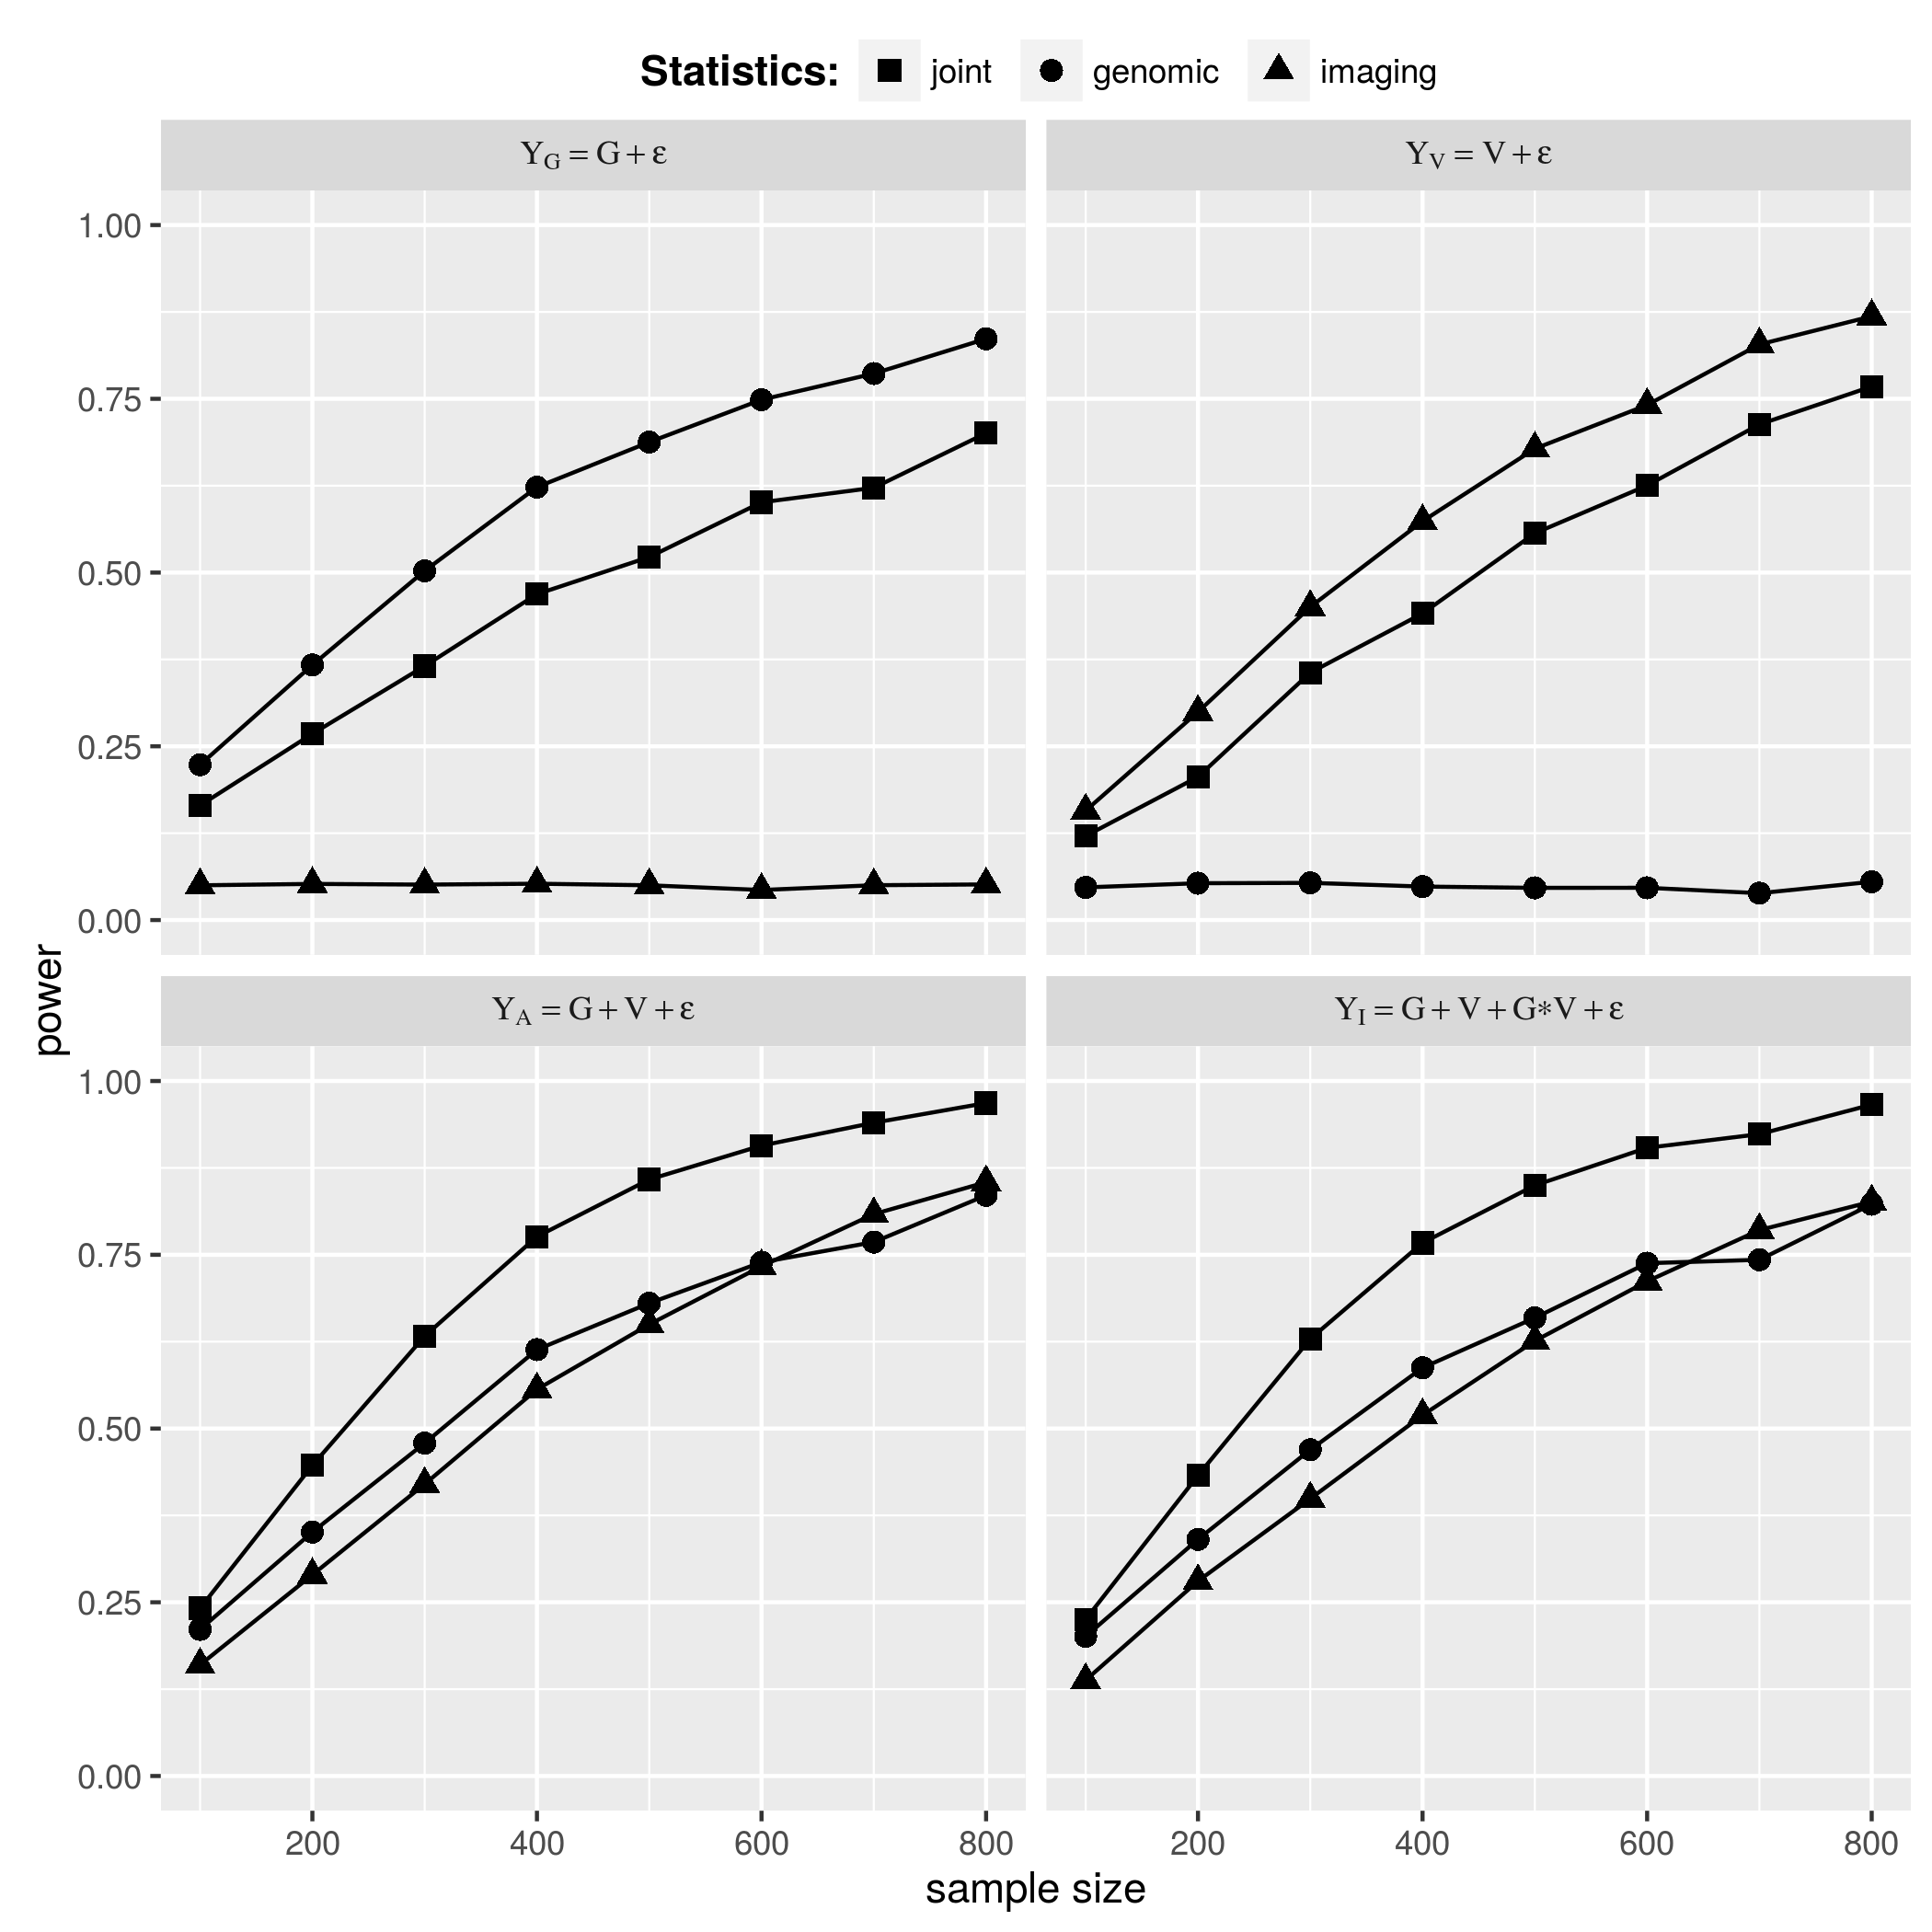
\includegraphics[width=300px]{PWR_CNT_KNL}
\caption{Robustness of the joint U statistic}
\end{figure}
The top row of Figure \ref{fig:PWR_CNT_KNL} shows that, the two parsimonious statistics $U_G$ and $U_V$ performed the best when the underlying effect is indeed purely genomic and vertex based, respectively, but they lost all the power when the actually consistuents of the effect do not concure with their choice of U-kernel functions. In constrast, the joint statistic $U_J$ performed fairly well under both circumstances, which is close to the power when the parsimonious kernel composition is correctly specified. What if the phenotipic variation is actually contributed by both genomic variants and cortical vertices? The bottom row of Figure \ref{fig:PWR_CNT_KNL} shows that, the joint statistic $U_J$ outperformed both $U_G$ and $U_V$ when the effect is additve, either with (Figure \ref{fig:PWR_CNT_KNL} down left) or without (Figure \ref{fig:PWR_CNT_KNL} down right) an additional interaction term.

\noindent \textbf{Grouping and Aggregation of Cortex Vertices} \\
Vertices in a cortex have no ``low MAF'' issue that rare genomic variants have, but the variant grouping and signal aggregation strategy adopted by deep sequencing study may still benefit analysis involving cortial surface. The second study aims to see if an aggregated cortex unit achieve higher power than the per-vertex based VWA followed by FDR (false discovery rate) correction. Comparison of the two strategy is done under the same 8 sample size and 4 effect composition scenarios except those with $U_G$ statistics, since cortex profile is not involved. The result is shown in Figure \ref{fig:PWR_CNT_VWA}.
\begin{figure}[!htbp]
\label{fig:PWR_CNT_VWA}
\centering
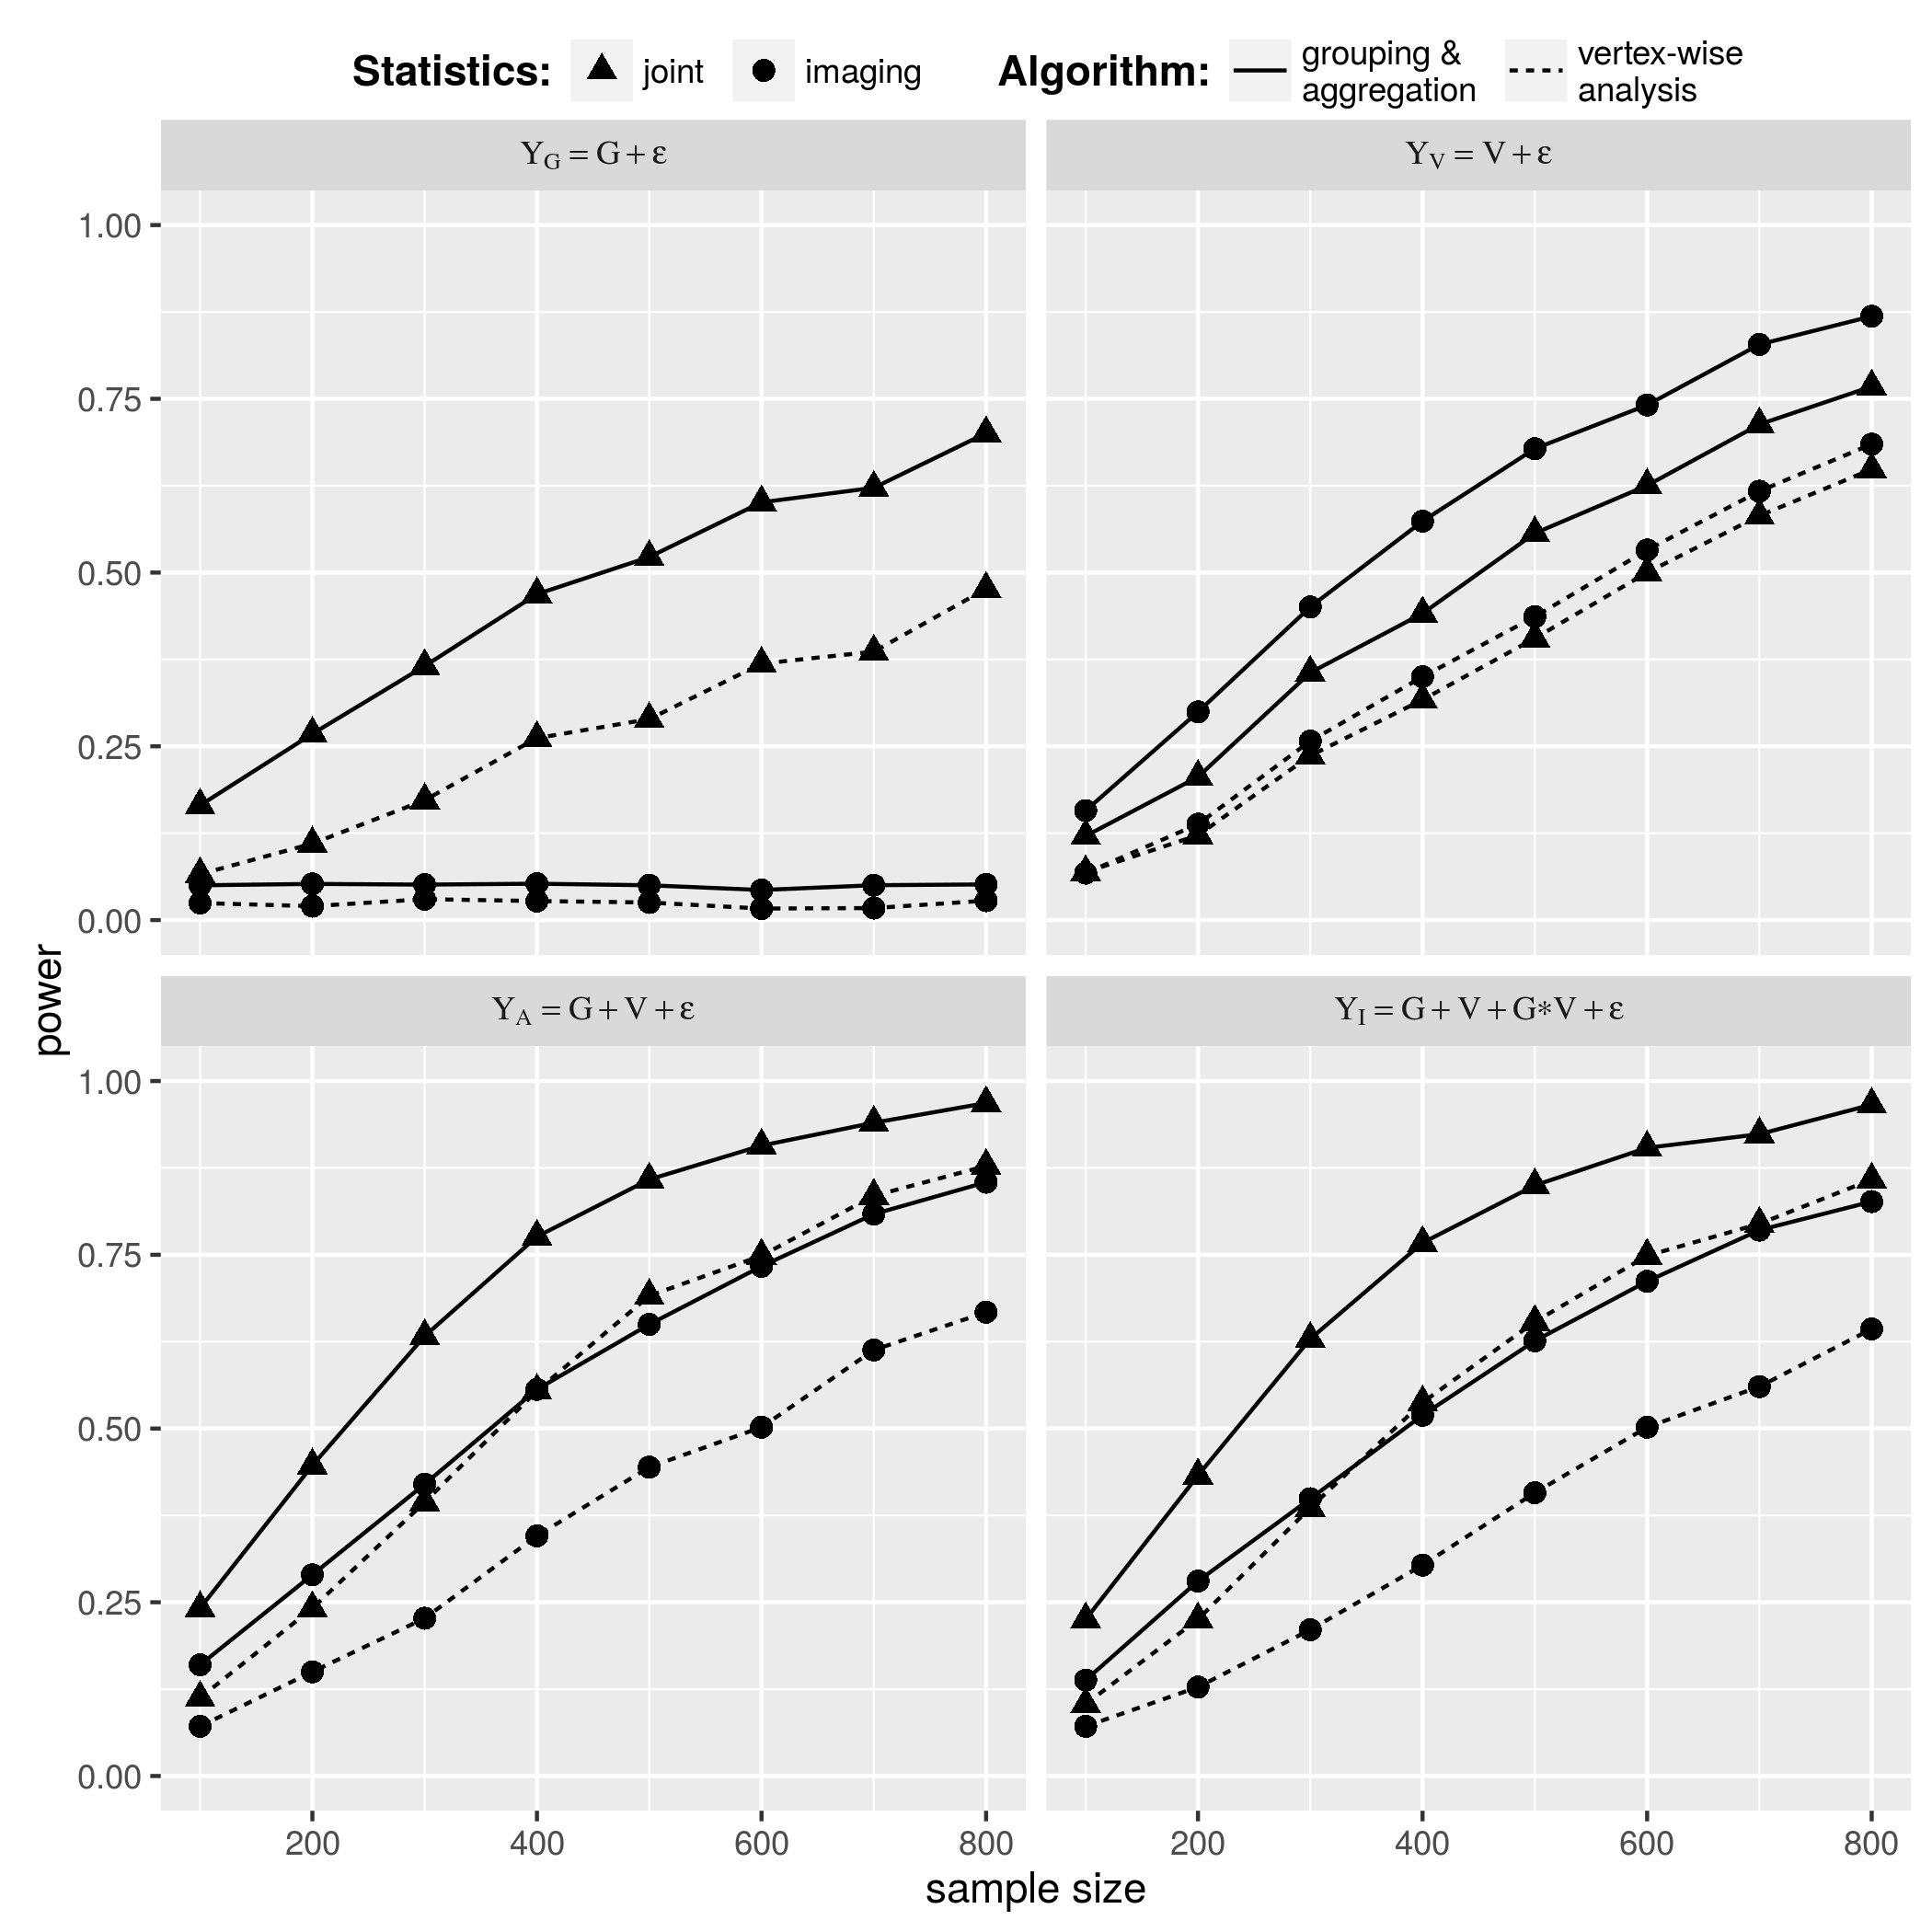
\includegraphics[width=300px]{PWR_CNT_VWA}
\caption{Grouping and Aggregation v.s. Vertex-wise Analysis}
\end{figure}
As we can see, under all simulation settings, the aggregated testing unit (solid lines) overpowers the per-vertex based VWA (dashed lines). This gap is only shortened when the sample size grows large. Another interesting speculation is the type I error rate of VWA is lower then the 0.05 threshold while the aggregated unit test is closely aligned to 0.05 (top left). The multiple testing correction is done by false discover rate (FDR) adjustment, which says that the adjusted p-value will be conservative if the tests were not independent. Therefore, a conservative type I error rate refects the fact that closely located vertices are correlated as they are sampling from tightly connected brain tissue. As a result, grouping and signal aggregation is also recommended for cortex profile.

\noindent \textbf{Abstract High Order Features from Cortex Vertices}
The third set of study tests whether the high order features abstracted from the raw cortex profile provides higher statistical power than the raw profile itself. Again the comparisons is done under all settings except those involving $U_G$ that doesn't rely on vertices in the cortex. The result is shown in Figure \ref{fig:PWR_CNT_SAE}.
\begin{figure}[!htbp]
\label{fig:PWR_CNT_SAE}
\centering
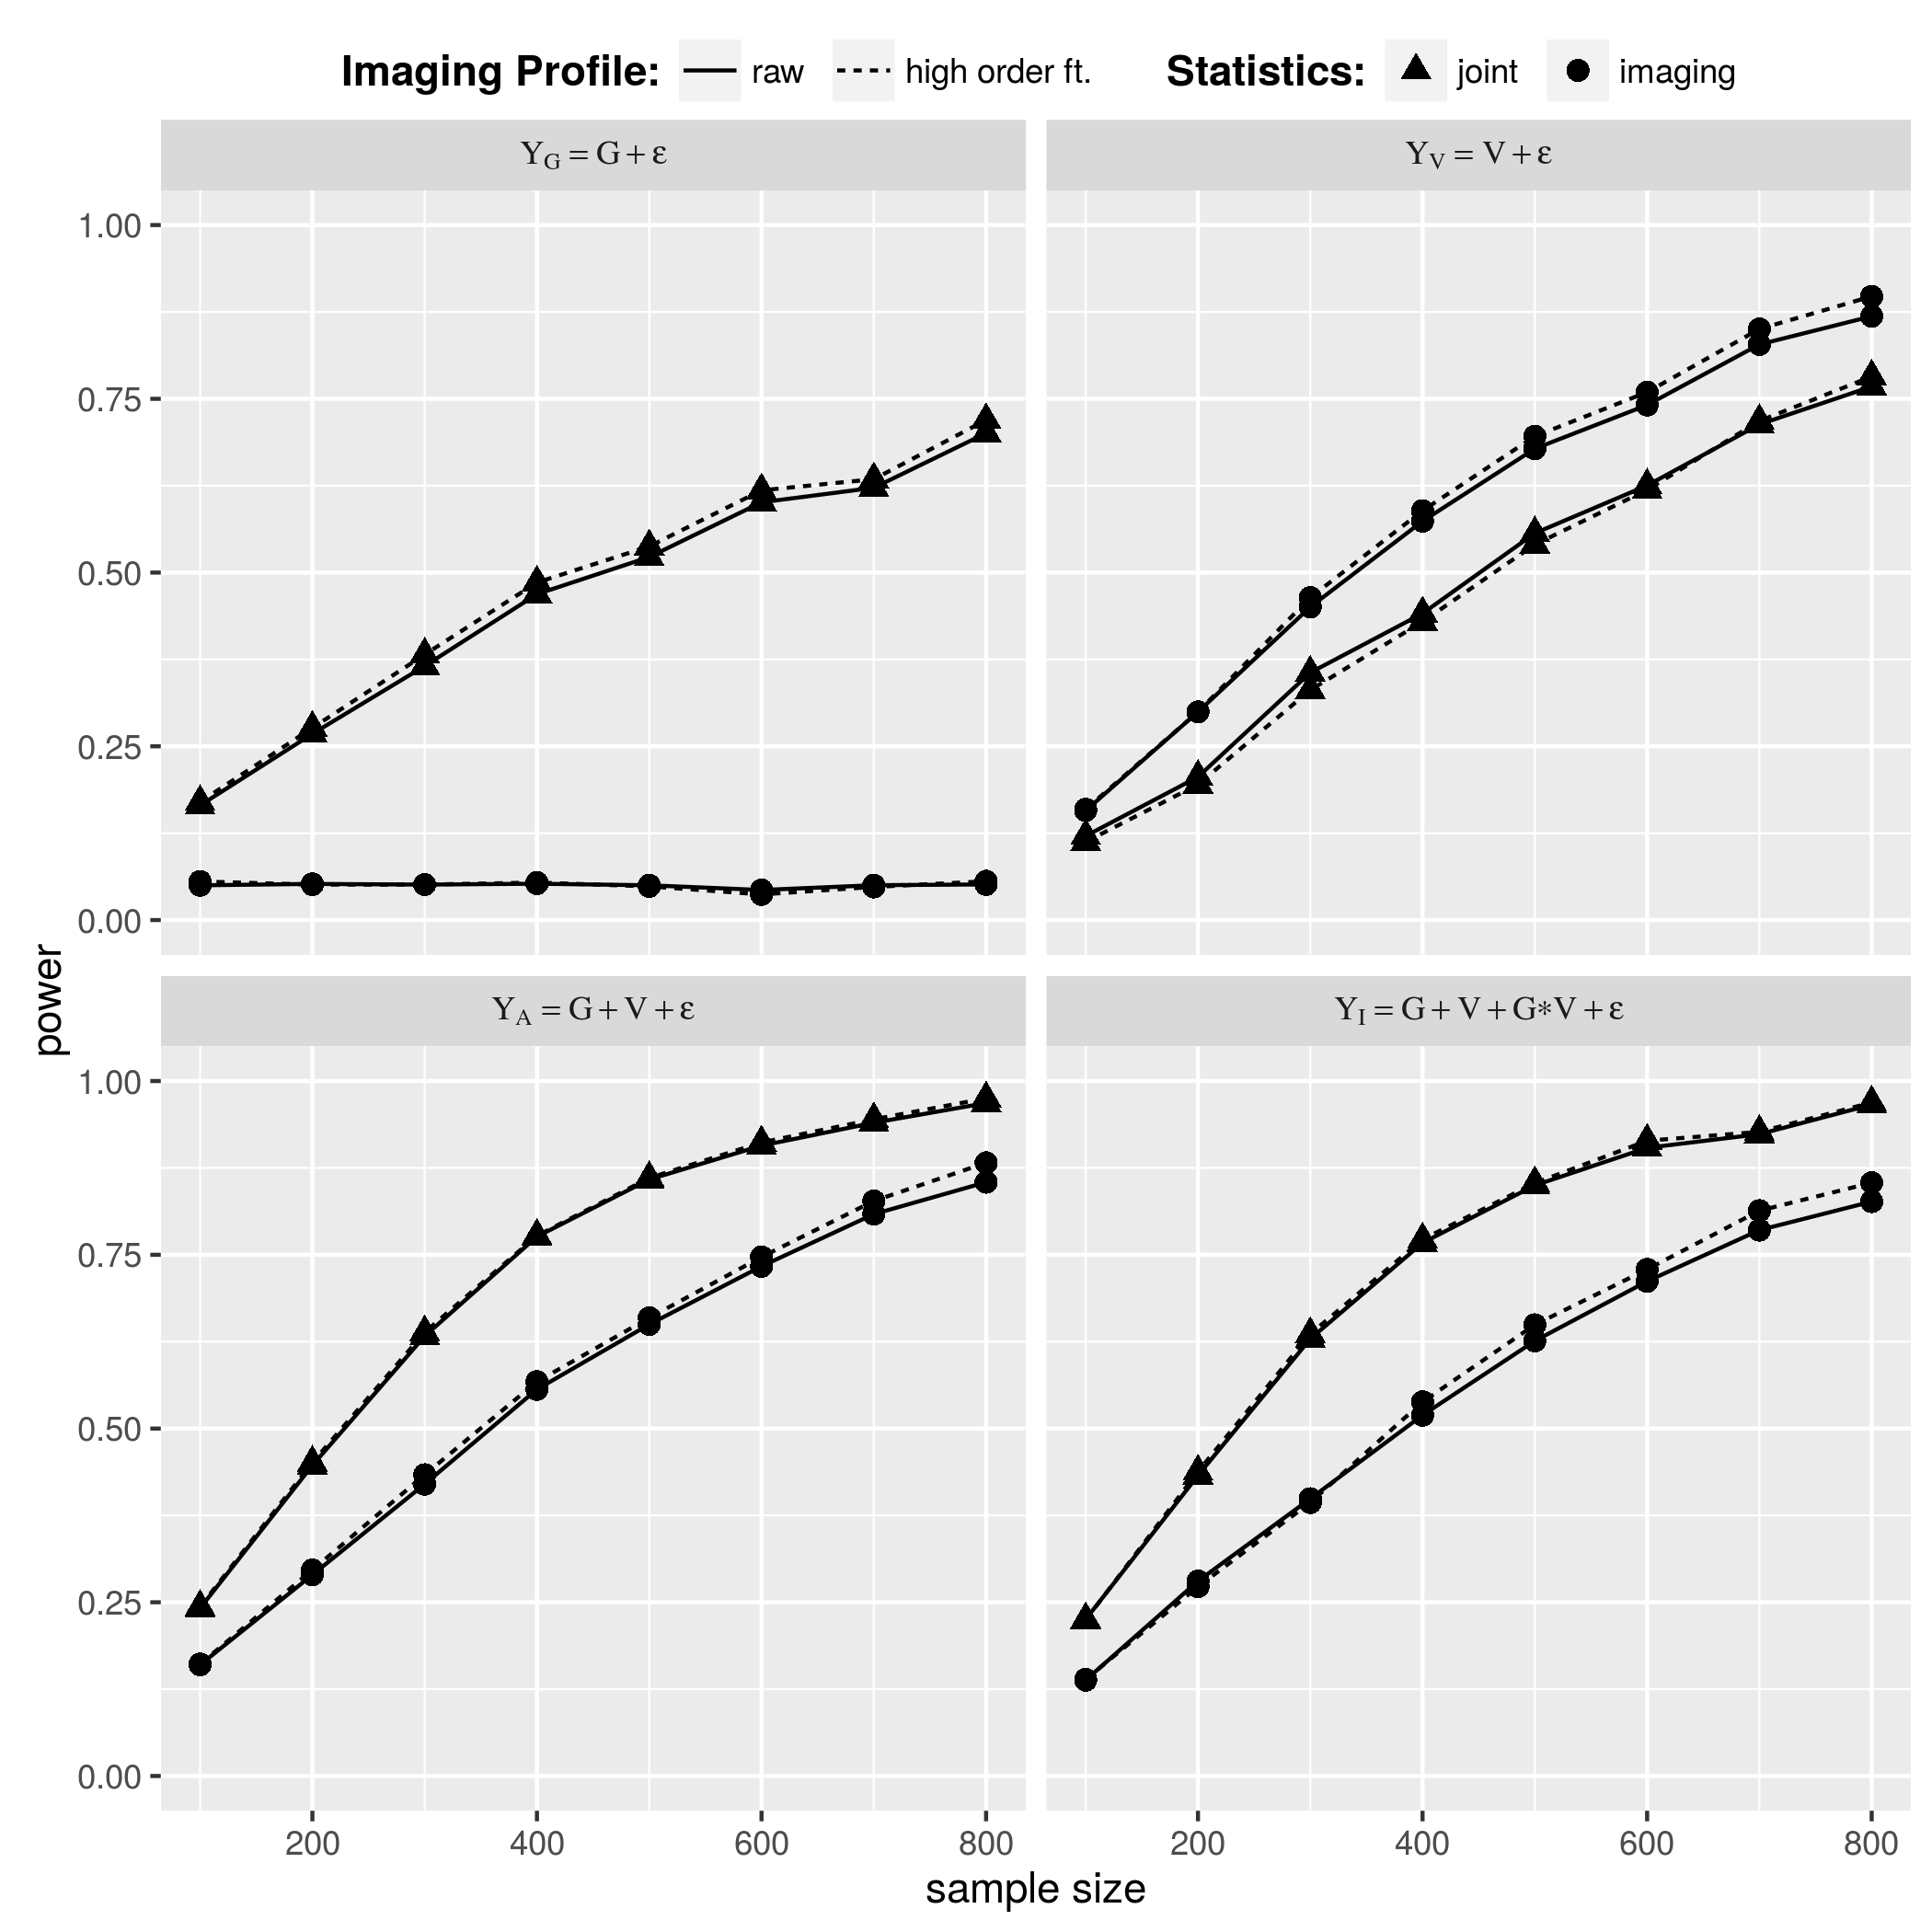
\includegraphics[width=300px]{PWR_CNT_SAE}
\caption{high order features v.s. raw vertices}
\end{figure}
In most scenarios, the abstracted features (Figure \ref{fig:PWR_CNT_SAE}, dashed lines) offers more power then the orignal vertices (Figure \ref{fig:PWR_CNT_SAE}, solid lines), and the edge is growing with the sample size become larger. The only exception happened when the sample size is lower then 600, the effect is purely vertex based, and the partially mis-specified joint U statistic is used for the test (Figure \ref{fig:PWR_CNT_SAE}, top right). Since the rejection of null hypothesis counts as type I error when the kernel functions are complete mis-sepcified, the top left panel in \ref{fig:PWR_CNT_SAE} shows that, the use of abstracted features doesn't deviate the type I error rate from the 0.05 threshold.

\textbf{Comparions using Dichotomous phenotypes}
The dichotomous responses is simulated by pluging the continuous responses into the inverse logit function for a set of probabilities, then draw the binary case/control status from these probabilities. The power performace shares very similar patterns under every scenario, albeit poorer then its continuous counterpart. The results is shown in Figure \ref{fig:PWR_BIN_KNL}, \ref{fig:PWR_BIN_VWA} and \ref{fig:PWR_BIN_SAE}.

In general, the simulation studies have so far demenstrated the robustness and versitility of the proposed method when faced with uncertain effect composition and a variety of phenotype distributions. Also shown is the helpfulness of groupping and aggregation strategy used by many rare genomic variant studies over other types of high dimenstional whose variants are not ``rare'' but potentlly correlated. The power boost offered by the stacked autoencoders is not dramatic, but is increasingly more positive when the sample size grows.

\section{Real Data Analysis}
The baseline data of 327 out of 806 participants who has definite diagnosis status entered the analysis. The genomic testing units are still defined by gene. The image testing units are now the 68 functional anatomy regions in the cortex. The 68 sets of vertices are piped into 68 stacked autoencoders trained with all 806 cortex profiles, and the resulting 68 sets of abstracted features are used to construct joint U statistic $U_J$. Among those 327 choosen subjects, 47 of them are diagnosed with either Alzheimer's disease (AD) or dementia, while the rest 280 subjests are healthy controls (CN). The case/control outcomes were first regressed on 7 known risk factors of AD, namely age, gender, race, ethnicity, years of education, marriage status, ever smoking, and APOE $\epsilon$4 haplotype. The regression residuals were then taken as the actual phenotype. For exploratory purpose, for each tuple of gene and cortex region, we also put the other two simplified statistics $U_G$ and $U_V$ into test. The testing resuls of 3 null hypothesis are show in Figure \ref{fig:RDA_PVL}, sorted from left to right by the p-value the joint U statistic $U_J$.
\begin{figure}[!htbp]
\label{fig:RDA_PVL}
\centering
\includegraphics[width=300px]{RDA_LGP}
\caption{p-values of real data analysis}
\end{figure}
Going through all triplets of $U_J$, $_G$ and $U_V$ statistics, we see most of the time, the joint statistic $U_J$ that involves a pair of gene and cortex region (Figure \ref{fig:RDA_PVL} dots), is less significant than the purely vertex based $U_G$ on the same cortex region (Figure \ref{fig:RDA_PVL} diamonds) but more significant than the purely genomic based statistic $U_G$ involves the same gene (Figure \ref{fig:RDA_PVL} cross). Such pattern reflects the facts that genomic effect is weak disease while the cortex profile is a strong indicator of the disease in the brain. From the whole picture, we see the joint statistcs ``borrowing'' information from the cortex profile, such that the p-values of $U_J$ align closer to the more significant $U_V$, and topple it when both $U_V$ and $U_G$ are significant for a pair of gene and cortex region.
The results showed that the vertex based test are statistically more significance then the genome based ones, which is coherent with the fact that the neuron loss and thinning of gray matter is an proxmate indicator of the progression of Alzheimer's , while genomic profile is a remote predictor of a greater uncertainty. A noteworthy phenominium is how the joint U statistic ($U_J$) could "borrow" power from the two simpler genomic ($U_G$) and vertex ($U_V$) statistics, such that for most combinations of gene and M regions the p-value of the joint test aligns closer to the more significant one of the two simpler U statistics, moreover, when both $U_G$ and $U_V$ are moderately significant, $U_J$ will be more so then either of them. In fact, the top 10 tests in table[?] were all from the joint U statistics $U_G$, which is the combination of the most significant WM region - left superiortemporal and the 10 most significant genes from tests $U_Vnnnn$ and $U_G$, respectively. Decection of left superiortemporal by either vertex U or joint U test is consistant with known fact that thinning of this region is a strong indicator for AD diagnosis, which is backed by ample evidences from imaging and atopsy studies [?]. The top genes so far detected couldn't remain statistically significant after multiple-testing correction and didn't contain or close to the top 20 SNPs [ref: AD SNP database] reported so far by GWAS and meta-analysis, they are likely to be due to chance.

20 most significant tuples, according to the smallest p value in each triplet of $U_J$, $U_G$ and $U_V$. 

% latex table generated in R 3.2.3 by xtable 1.7-4 package
% Thu Feb 11 21:19:43 2016
\begin{table}[ht]
\centering
\begin{tabular}{lllll}
  \hline
  cortex & gene & $P_V$ & $P_G$ & $P_X$ \\ 
  \hline
  SFG & IGLV1-44 & 1.68e-11 & 3.51e-04 & 2.77e-13 \\ 
  SFG & NBEAP2 & 1.68e-11 & 1.19e-04 & 4.74e-13 \\ 
  SFG & RPL21P89 & 1.68e-11 & 6.36e-04 & 5.14e-13 \\ 
  SFG & LOC102724504 & 1.68e-11 & 1.41e-03 & 5.56e-13 \\ 
  SFG & CNTNAP3P8 & 1.68e-11 & 1.08e-03 & 6.17e-13 \\ 
  SFG & CDH4 & 1.68e-11 & 4.64e-03 & 6.96e-13 \\ 
  SFG & HNRNPA1P19 & 1.68e-11 & 8.88e-04 & 7.80e-13 \\ 
  SFG & FAM72C & 1.68e-11 & 9.28e-06 & 7.82e-13 \\ 
  SFG & RP11-638L3.1 & 1.68e-11 & 1.41e-01 & 9.49e-13 \\ 
  SFG & CPXM1 & 1.68e-11 & 8.78e-04 & 1.08e-12 \\ 
  SFG & LOC101929612 & 1.68e-11 & 1.44e-02 & 1.15e-12 \\ 
  SFG & LOC100996517 & 1.68e-11 & 6.77e-04 & 1.20e-12 \\ 
  SFG & IGLV5-45 & 1.68e-11 & 3.44e-04 & 1.23e-12 \\ 
  SFG & MIS18BP1 & 1.68e-11 & 4.95e-03 & 1.35e-12 \\ 
  SFG & CDR2 & 1.68e-11 & 1.82e-04 & 1.39e-12 \\ 
  SFG & RPL41P2 & 1.68e-11 & 6.04e-03 & 1.59e-12 \\ 
  SFG & LOC101927737 & 1.68e-11 & 7.20e-03 & 1.60e-12 \\ 
  SFG & IGLV1-47 & 1.68e-11 & 1.44e-02 & 1.60e-12 \\ 
  SFG & IGLV7-46 & 1.68e-11 & 9.15e-04 & 1.69e-12 \\ 
  SFG & ZDHHC15 & 1.68e-11 & 1.56e-03 & 1.73e-12 \\ 
   \hline
\end{tabular}
\caption{Top 20 combinations} 
\label{tb:tp20}
\end{table}


